\section{Fault Model Analysis in the Shared Model Process}
\label{sec:fault_analysis_2}

To demonstrate the shared model process, we outline a subsystem of the WBS and describe the interaction between system development process and the system safety process using a shared model. The AIR6110 document provides a detailed example of the aircraft and systems development for a function of a hypothetical S18 aircraft and we will refer to this standard throughout this section. What we wish to accomplish is to show how the model based process and the use of the Safety Annex fits into this development. 

Initially in the development of a critical system, the planning documents define the developmental process activity. This provides description of the system in question (i.e. the aircraft which holds the wheel brake system) and leads to the aircraft preliminary design. The functions of the aircraft are defined and decomposed, in this case, into the functional statement of this subsystem: "Decelerate aircraft on the ground." The top level requirements are decomposed and pertinant requirements for this subsystem are found. 

Given that the functional requirements of the subsystem are now defined, the preliminary model of the WBS subsystem can be developed on the system engineering side of the process (refer to figure used in prelim section outlining this process). The safety analysis development takes those functions and develops a Functional Hazard Assessment based on them. As an example, we look at one possible hazard based on the top level aircraft requirement: "Aircraft shall have a means to decelerate on the ground." The aircraft level function is then "Decelerate on the ground." This is broken down into two main functions of the WBS: (1) Provide primary stopping force and (2) Provide secondary stopping force. \danielle{This process/paragraph needs help... clarification.}

The preliminary system model is built using AADL, the requirements are decomposed into individual subcomponent contracts constraining output behavior and assumptions on input values.  

\subsection{Nominal Model Analysis Example}
Given the top level requirements, the architecture of the system must reflect the necessary behavior in order to meet these requirements. Before fault analysis can proceed, the nominal model (behavior in the absence of faults) must be verified and the requirements must be met. Using the AADL model, we go through a brief example to illustrate how lower level subcomponent contracts can support the requirement that was discussed in Section \ref{sec:fault_modeling}: Inadvertent braking. Figure 4 shows the AGREE form of this requirement. 

\begin{figure}[h!]
	\vspace{-0.2in}
	\begin{center}
		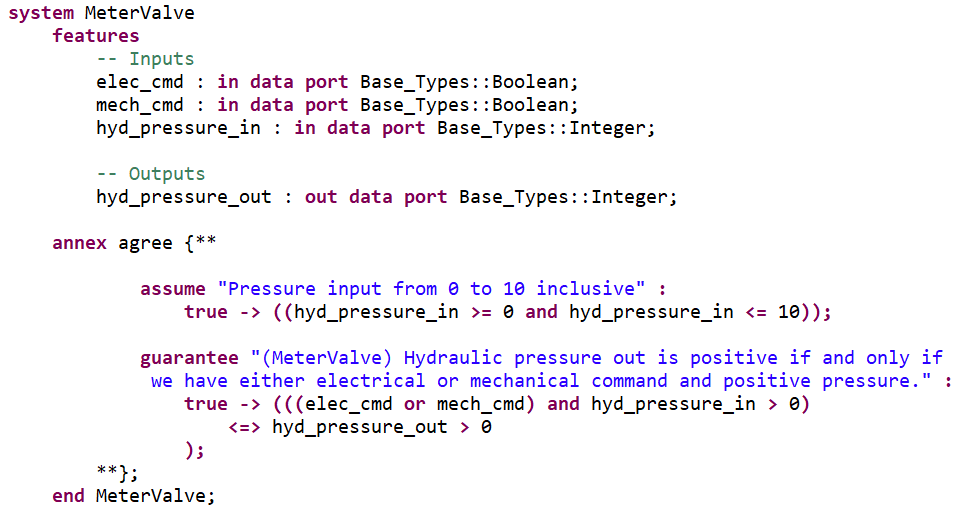
\includegraphics[width=0.8\textwidth]{images/metervalve.png}
	\end{center}
	\vspace{-0.3in}
	\caption{AADL and AGREE Subcomponent: Meter Valve}
	\label{fig:metervalve}
	%\vspace{-0.2in}
\end{figure} 

If power and pressure are supplied while the wheel is rolling and ground speed is positive \textit{and the pedal is not pressed}, then braking force is zero. This dictates that there must be a subcomponent that shuts off the hydraulic pressure to the wheel brake when the pedal is not being pressed. In this architecture, this is the Meter Valve subcomponent. As shown in Figure
\ref{fig:wbs}, the Meter Valve takes input from the Control System (the pedal command) and the Selector Valve (hydraulic pressure line). The contracts of this component support the inadvertent braking contract by stating that if the pedal is pressed and hydraulic pressure is supplied, then the hydraulic output of the Meter Valve is positive. The AADL and AGREE code is shown in Figure \ref{fig:metervalve}. 

 

\subsection{Fault Model Analysis Example}
Now that the initial architecture is made in AADL and the nominal model proves using AGREE/JKind, the preliminary system safety assessment (PSSA) begins looking at the WBS subsystem and attempts to identify possible faults for the subcomponents using the hazard analysis as a guide. The PSSA assesses how failures can lead to the associated functional hazards of the aircraft FHA by identifying the elements and interactions that contribute to the relevant failure conditions. Utilizing the shared architectural and behavioral model, the assessment can focus on how various subcomponents can fail. These are then inserted into the model using the Safety Annex, and analysis can run. This analysis provides the necessary artifacts for the PSSA (e.g. fault trees, probabilities, etc.). 

To illustrate this, we continue the example from the previous section regarding inadvertent braking. The safety analysts comb through the subcomponents of the system and find common types of failures. For instance, in this WBS model, there are sensors on the mechanical brake pedals. These sensors transmit a digital signal when the brakes are pressed. This signal is passed to the control system and BSCU which then propagate the command for braking. Imagine the particular sensor in use will have a failure rate of $5 \times 10^{-6}$ per flight hour. The analyst will insert the fault as shown in Figure \ref{fig:sensorFault}. 

\begin{figure}[h!]
	\hspace*{-2cm}
	\vspace{-0.5in} 
	\begin{center}
		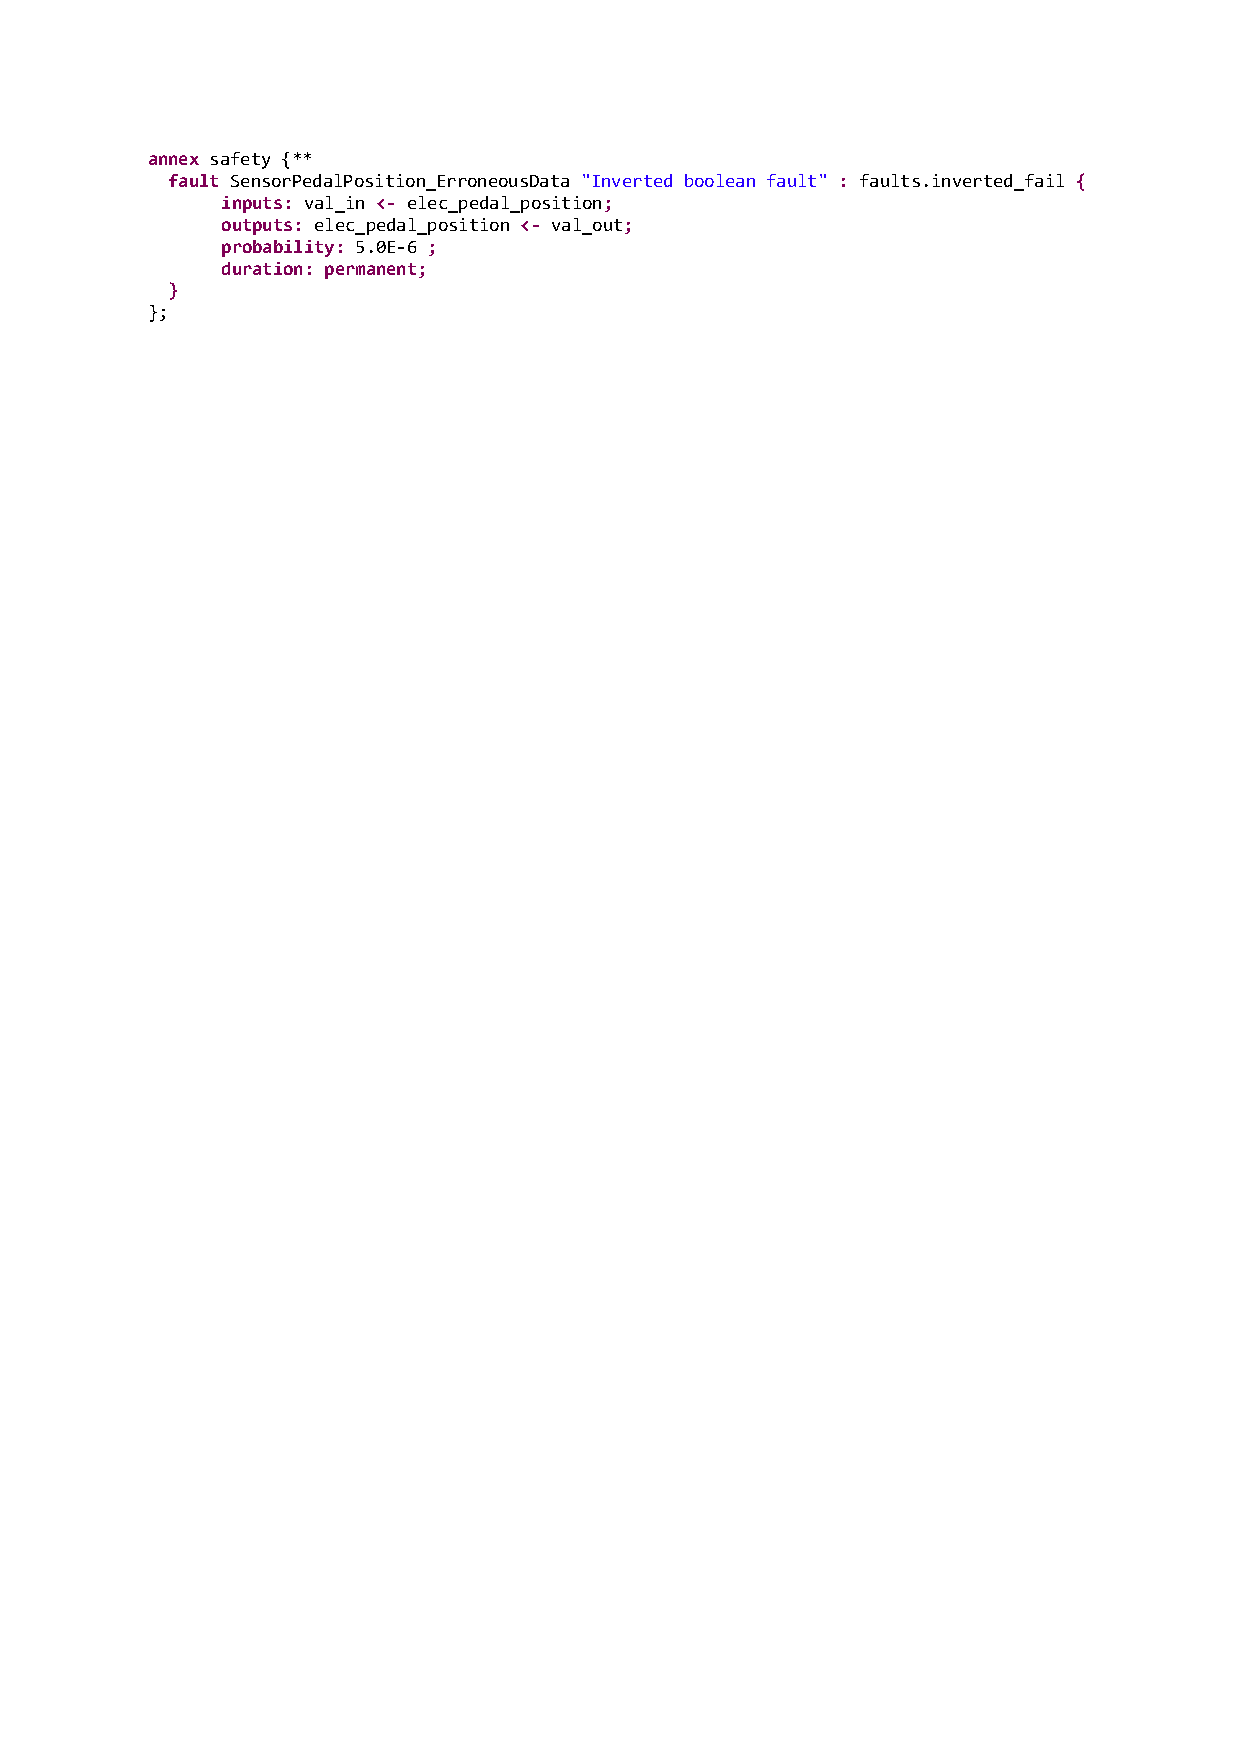
\includegraphics[trim=0 680 -10 70,clip,width=1.5\dimexpr\textwidth-2cm\relax]{images/safetyannex_sensorfault.pdf}
		%\vspace{-0.3in}
		\caption{The Safety Annex for the Pedal Sensor}
		\label{fig:sensorFault}
	\end{center}
	\vspace{-0.3in}
\end{figure}

These faults are then modeled using the Safety Annex and the same AADL/AGREE model that was used in the system architecture development side. Simultaneously, the system probability allocations are determined and factored into the fault analysis. The results from the analysis can then provide information on both the component failures that contribute to a hazard and the probability of such occurrences. Given the results from the analysis, the analyst then flags certain subcomponents or architectural decisions for reconsideration. 

\begin{figure}[h!]
	\vspace{-0.2in}
	\begin{center}
		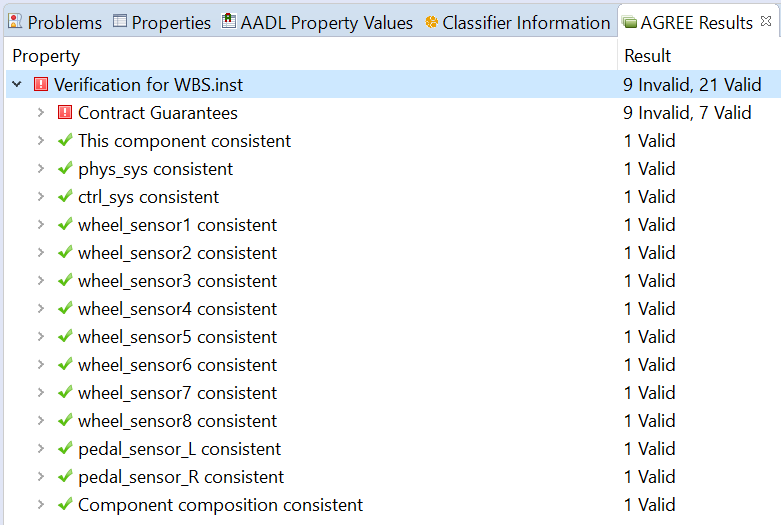
\includegraphics[width=0.8\textwidth]{images/agreeResults.png}
	\end{center}
	\vspace{-0.3in}
	\caption{Results in AGREE after running fault analysis}
	\label{fig:agreeResults}
	%\vspace{-0.2in}
\end{figure}

The fault analysis run on the top system level is shown in Figure \ref{fig:agreeResults}. The top level properties are shown to be false with max 1 fault analysis. 

\begin{figure}[h!]
	\vspace{-0.2in}
	\begin{center}
		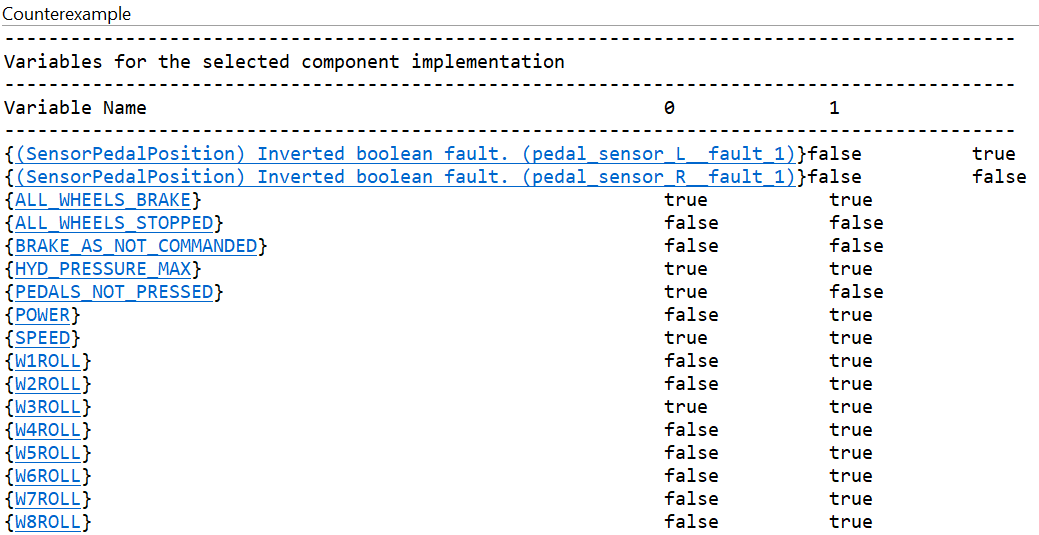
\includegraphics[width=0.8\textwidth]{images/pedalCoEx.png}
	\end{center}
	\vspace{-0.3in}
	\caption{Counterexample Showing Active Fault}
	\label{fig:coEx}
	%\vspace{-0.2in}
\end{figure}

Viewing the counterexample shows the fault that is active which causes this problem to occur (Figure \ref{fig:coEx}).

Given these results from the analysis, the archtecture can be changed to make this subsystem of the WBS more resiliant to faults and hence better support the top level requirements of the aircraft. \danielle{Make architectural adjustments with code snippets and figure adjustments to clarify how the system is changed.}

Using this same model, the safety analysis must only be rerun to determine the impact of changes to the system model. \danielle{Show new analysis results.} 

As can be seen through this single example, a system as large as the WBS would benefit from many iterations of this process. Furthermore, if the model is changed even slightly on the system development side, it would automatically be seen from the safety analysis perspective and any negative outcomes would be shown upon subsequent analysis runs. This effectively eliminates any miscommunications between the development and analysis teams and creates a new safeguard regarding model changes. 

\danielle{To end the section, summarize the key points: how we fit into the process and why it matters. Perhaps mention that this is only a small example of what can be modeled using the safety annex and for more information about modeling capabilities, look at the users guide.}


